\documentclass[sigconf,anonymous,review]{acmart}

\setcopyright{none}
\settopmatter{printacmref=false,printfolios=true}
\acmConference[WSDM '27]{ACM International Conference on Web Search and Data Mining}{2027}{}
\acmBooktitle{ACM International Conference on Web Search and Data Mining (WSDM '27)}

\begin{CCSXML}
<ccs2012>
 <concept><concept_id>10010147.10010257</concept_id><concept_desc>Computing methodologies~Machine learning</concept_desc><concept_significance>500</concept_significance></concept>
 <concept><concept_id>10002951.10003260</concept_id><concept_desc>Information systems~Web searching and information discovery</concept_desc><concept_significance>300</concept_significance></concept>
</ccs2012>
\end{CCSXML}
\ccsdesc[500]{Computing methodologies~Machine learning}
\ccsdesc[300]{Information systems~Web searching and information discovery}

% Generated by experiments.paper_export. Do not hand-edit.
\providecommand{\PaperStatus}{Not run}
\providecommand{\SourceTrainCount}{5611}
\providecommand{\SourceValidationCount}{1402}
\providecommand{\FHMTestCount}{9000}
\providecommand{\OursFHMMacroFOne}{\texttt{TBD}}
\providecommand{\BestBaselineName}{\texttt{TBD}}
\providecommand{\OursImprovement}{\texttt{TBD}}
\providecommand{\PaperDraftPlaceholder}[1]{\textit{[Draft status: #1]}}


\begin{document}
\title{Evidence-Grounded Harmful Meme Interpretation Across Domains}
\author{Anonymous Authors}

\begin{abstract}
Harmful memes often express abuse through subtle interactions between images
and overlaid text, and their interpretation may depend on implicit social,
cultural, and event-specific knowledge. Existing methods largely focus on
binary detection, leaving targets, intents, rhetorical strategies, and
supporting evidence implicit. We formulate harmful meme understanding as a
structured interpretation task that jointly predicts harmfulness, target
presence and granularity, primary intent, rhetorical tactics, and image--text
relations. Our five-stage framework extracts global, local, textual, and
cross-modal evidence; acquires external knowledge candidates; verifies their
relevance, validity, and task-specific support; fuses internal evidence with
verified knowledge through task-aware reasoning; and outputs structured
predictions with evidence attribution and a concise rationale. A masked
multi-task objective supports partially available labels, while provenance
records distinguish retrieved documents, generated hypotheses, verified
evidence, and rejected candidates. We train and validate on HarMeme and
evaluate generalization on the held-out Facebook Hateful Memes benchmark under
a leakage-controlled protocol. Beyond harmfulness detection, we separately
assess target, intent, and tactic using schema-validated silver annotations
with field-level coverage. This setup enables a unified evaluation of
cross-domain detection, multi-dimensional interpretation, and auditable
evidence-grounded reasoning.
\end{abstract}

\keywords{harmful memes, multimodal reasoning, evidence attribution, cross-domain evaluation}
\maketitle

% !TeX root = ../main.tex
\section{Introduction}
\label{sec:introduction}

Memes combine images and short text to convey meaning through cultural
references, visual symbolism, sarcasm, and other forms of multimodal
composition.  The same properties make harmful memes difficult to detect:
an image or sentence may appear benign in isolation while their combination
targets a person or group, expresses an abusive intent, or invokes a
harmful rhetorical strategy.  Effective moderation therefore requires more
than recognizing unimodal surface cues.

Prior work has addressed binary harmful or hateful meme detection with
multimodal representations, cross-modal interaction, and
contrastive learning~\cite{kiela2020hateful,kumar2022hateclipper,shah2024memeclip,mei2024rgcl}.
More recent methods have begun to predict targets or attack types and to
generate natural-language rationales~\cite{pramanick2021harmeme,sharma2022disarm,lin2024explainhm}.
These advances
move toward richer meme understanding, but fine-grained prediction,
evidence grounding, and rationale generation are still often treated as
separate or method-specific outputs.  We instead formulate harmful meme
understanding as a structured interpretation task that jointly predicts
harmfulness, target presence and granularity, primary intent, rhetorical
tactics, and multimodal relation.

A second challenge is that the meaning of a meme may depend on social,
cultural, or event-specific context that is not directly observable in its
pixels or OCR text.  Retrieval and multimodal language models can provide
such context, but acquired information is not automatically reliable
evidence.  Retrieved examples may be only superficially similar, generated
hypotheses may be unsupported, and context relevant to identifying a target
may not support the same conclusion about intent or rhetorical strategy.
This motivates our central design question: \emph{how should external
knowledge be checked against the meme before it is allowed to influence a
structured prediction?}

We propose an evidence-grounded framework that explicitly separates
knowledge acquisition from evidence verification.  Internal evidence is
extracted from global and local visual content, OCR text, and image--text
interaction, while external candidates are acquired when additional context
is useful.  Before fusion, an evidence-aware verifier evaluates each
candidate against the internal meme evidence for relevance, validity, and
task-specific support.  Only verified knowledge enters task-aware
reasoning; accepted and rejected candidates retain their provenance for
analysis.  The final model outputs the structured predictions together with
selected evidence and a concise rationale.

We evaluate cross-domain generalization by developing models exclusively on
HarMeme~\cite{pramanick2021harmeme,pramanick2021momenta} and testing them on
the held-out Facebook Hateful Memes benchmark
(FHM)~\cite{kiela2020hateful}.  No FHM example is used for model selection, prompt development, or
retrieval construction.  Beyond harmfulness, schema-validated silver
annotations enable evaluation of target, intent, rhetorical tactics, and
multimodal relation under the same domain shift.

Our contributions are threefold:
\begin{itemize}
    \item
    We formulate harmful meme understanding as structured prediction over
    harmfulness, target presence and granularity, primary intent,
    rhetorical tactics, and multimodal relation.

    \item
    We introduce an evidence-aware verification stage that evaluates
    externally acquired candidates against internal meme evidence for
    relevance, validity, and task-specific support before they can
    influence downstream multimodal reasoning.

    \item
    We conduct a cross-domain evaluation from HarMeme to FHM with
    specialized harmful-meme models and general-purpose vision--language
    baselines, and analyze structured transfer, component contributions,
    and external-knowledge filtering behavior.
\end{itemize}

% !TeX root = ../main.tex
\section{Related Work}
\label{sec:related_work}

\subsection{Harmful Meme Detection and Structured Understanding}
\label{sec:related:detection}

Harmful and hateful meme detection is inherently multimodal because the
harmful meaning may emerge only from the interaction between an image and
its accompanying text.
The Hateful Memes benchmark~\cite{kiela2020hateful} helped establish this setting, and subsequent
work has explored stronger multimodal fusion and pretrained
vision--language representations.
CLIP-based methods such as HateCLIPper~\cite{kumar2022hateclipper} and
MemeCLIP~\cite{shah2024memeclip} model image--text
interactions for meme classification, while MOMENTA combines global and
local multimodal evidence and extends detection toward harmful-target
identification~\cite{pramanick2021momenta}.
Related approaches such as DISARM~\cite{sharma2022disarm} likewise emphasize identifying victims
or targets rather than predicting harmfulness alone.

Recent work increasingly moves beyond a single binary label.
SAFE-MEME~\cite{nandi2024safememe} uses structured question--answer reasoning and hierarchical
categorization, including questions about the target and type of hate.
EXPLAINHM~\cite{lin2024explainhm} and
EXPLAINHM++~\cite{lin2026explainhmpp} generate natural-language rationales through
multimodal debate, and recent large-multimodal-model approaches such as
RA-HMD~\cite{mei2025rahmd} and ExPO-HM~\cite{mei2026expohm} incorporate fine-grained supervision, reasoning, or
explanation into harmful-meme modeling.
These developments motivate richer outputs, but target prediction,
fine-grained categorization, rationale generation, and evidence grounding
are still often represented as method-specific objectives.
Our formulation instead places harmfulness, target presence and
granularity, primary intent, rhetorical tactics, and multimodal relation in
one structured prediction space, while retaining a separate evidence record
for audit.

\subsection{Knowledge-Augmented Meme Reasoning}
\label{sec:related:knowledge}

Meme interpretation can depend on social, cultural, and event-specific
knowledge that is absent from the pixels or OCR text.
PromptHate introduces image-derived textual context into prompt-based
classification, whereas retrieval-based methods explicitly introduce
related examples or documents~\cite{cao2022prompthate}.
RGCL~\cite{mei2024rgcl} uses retrieved meme relationships for contrastive representation
learning and retrieval-based inference, and RA-HMD combines multimodal
adaptation with retrieval-oriented representations for out-of-domain
classification.
EXPLAINHM++ retrieves related harmful and harmless memes to ground a second
round of multimodal debate before producing its final decision and
rationale.

A closely related issue is robustness to noisy retrieval.
MerFT~\cite{lee2026merft} studies distractor-aware multimodal meme
reasoning and trains retrieval-augmented models to remain robust to
semantically plausible but misleading documents.
Its experiments explicitly vary distractor frequency, demonstrating that
retrieval quality can materially affect meme reasoning.
This reinforces the need to treat retrieved context as potentially noisy
rather than inherently trustworthy.

Our focus is complementary but different.
Instead of relying only on retrieval-aware training to become robust to
distractors, we place an explicit candidate-level verifier between
knowledge acquisition and multimodal fusion.
Each external candidate is evaluated against internal meme evidence for
relevance, validity, and task-specific support before it can influence the
structured prediction.
The framework additionally retains both accepted and rejected provenance,
allowing retrieval quality and verification behavior to be analyzed
separately.
Thus, the central distinction of our approach is not retrieval itself, but
the explicit conversion of acquired context into \emph{verified evidence}
before task-aware reasoning.

\section{Problem Formulation}
\label{sec:problem}

\subsection{Structured Harmful Meme Interpretation}
\label{sec:problem:task}

A meme is a multimodal instance
$\mathcal{M}=(I,T)$, where $I$ denotes the meme image and
$T$ denotes the text extracted from the image using optical
character recognition.
Conventional harmful meme detection predicts a binary label from
$\mathcal{M}$.
In contrast, we formulate meme understanding as a structured
interpretation problem that jointly identifies whether the meme is
harmful, who or what it targets, what communicative intent it
expresses, and which rhetorical and multimodal strategies construct
its meaning.

For each meme, the model predicts

\begin{equation}
\hat{\mathcal{Y}}
=
\left(
\hat{y}^{h},
\hat{y}^{p},
\hat{y}^{g},
\hat{y}^{i},
\hat{\mathbf{y}}^{r},
\hat{y}^{m}
\right),
\label{eq:structured_output}
\end{equation}

where $\hat{y}^{h}$ is the harmfulness prediction,
$\hat{y}^{p}$ denotes target presence,
$\hat{y}^{g}$ denotes target granularity,
$\hat{y}^{i}$ is the primary communicative intent,
$\hat{\mathbf{y}}^{r}$ is a multi-label prediction over rhetorical
tactics, and $\hat{y}^{m}$ denotes the multimodal relation through
which the image and text jointly convey meaning.

Harmfulness, target presence, target granularity, primary intent,
and multimodal relation are modeled as single-label classification
tasks.
Rhetorical tactic prediction is modeled as a multi-label task
because a meme may simultaneously employ multiple strategies, such
as sarcasm, stereotyping, dehumanization, or exaggeration.
Task-specific labels denoting insufficient or ambiguous supervision
are excluded using field-level masks, whereas a valid
\texttt{none} category is retained when the corresponding
phenomenon is absent.

\subsection{Evidence-Grounded Interpretation}
\label{sec:problem:evidence}

A structured label alone does not explain why a meme is considered
harmful.
We therefore require the framework to retain the evidence and
knowledge used to produce its predictions.
Let

\begin{equation}
\mathcal{E}^{\mathrm{int}}
=
\left\{
e^{\mathrm{text}},
e^{\mathrm{visual}},
e^{\mathrm{cross}}
\right\}
\label{eq:internal_evidence}
\end{equation}

denote internal evidence extracted directly from the meme.
It may include relevant OCR spans, visual entities or regions, and
cross-modal cues arising from the interaction between the image and
text.

The framework may additionally acquire a set of external contextual
candidates,

\begin{equation}
\mathcal{C}^{\mathrm{ext}}
=
\left\{
c_1,\ldots,c_K
\right\},
\end{equation}

from retrieval, context generation, or fallback mechanisms.
These candidates are not assumed to be reliable evidence.
A verifier evaluates their relevance, validity, and task-specific
support, producing a verified subset

\begin{equation}
\mathcal{E}^{\mathrm{ver}}
=
\mathcal{V}
\left(
\mathcal{M},
\mathcal{E}^{\mathrm{int}},
\mathcal{C}^{\mathrm{ext}}
\right)
\subseteq
\mathcal{C}^{\mathrm{ext}},
\label{eq:verified_evidence}
\end{equation}

where $\mathcal{V}$ denotes the verification procedure.
Retrieved candidates, generated hypotheses, fallback candidates,
verified evidence, and rejected candidates remain explicitly
distinguished through provenance metadata.

The final output therefore consists of both the structured
prediction in Eq.~\eqref{eq:structured_output} and an explanatory
record

\begin{equation}
\hat{\mathcal{A}}
=
\left(
\mathcal{E}^{\mathrm{int}},
\mathcal{E}^{\mathrm{ver}},
\mathcal{P},
\hat{R}
\right),
\label{eq:explanation_output}
\end{equation}

where $\mathcal{P}$ represents evidence and decision provenance and
$\hat{R}$ is a concise rationale grounded in the selected evidence.
The rationale is an explanatory output rather than a substitute for
the task predictions, and it should not introduce claims unsupported
by either the meme or the verified contextual evidence.

\subsection{Multi-Task Learning Objective}
\label{sec:problem:objective}

Let
$\mathcal{Q}=\{h,p,g,i,r,m\}$ denote the set of prediction tasks.
For sample $n$ and task $q$, let $m_n^q\in\{0,1\}$ be a supervision
mask indicating whether a valid label is available.
Let $w_n$ denote a sample weight derived from annotation-quality
metadata, and let $\lambda_q$ denote the task weight.
The overall learning objective is

\begin{equation}
\mathcal{L}(\theta)
=
\frac{1}{N}
\sum_{n=1}^{N}
w_n
\sum_{q\in\mathcal{Q}}
\lambda_q m_n^q
\,
\ell_q
\left(
f_\theta^q(\mathcal{M}_n),
y_n^q
\right),
\label{eq:multitask_objective}
\end{equation}

where $f_\theta^q$ is the prediction function for task $q$.
We use single-label classification losses for
$q\in\{h,p,g,i,m\}$ and a multi-label binary classification loss for
$q=r$.
This masked objective permits the framework to learn from partially
available structured supervision without treating missing or
ignored labels as negative instances.

\subsection{Cross-Dataset Generalization}
\label{sec:problem:generalization}

We study a source-to-target generalization setting.
The source collection

\begin{equation}
\mathcal{D}_{S}
=
\mathcal{D}_{\mathrm{COVID}}
\cup
\mathcal{D}_{\mathrm{Politics}}
\end{equation}

combines the COVID-19 and U.S.\ politics domains of HarMeme while
preserving their original domain identities.
It is partitioned into a source training set
$\mathcal{D}_{S}^{\mathrm{train}}$ and a source validation set
$\mathcal{D}_{S}^{\mathrm{val}}$.
The Facebook Hateful Memes collection forms a disjoint held-out
target set $\mathcal{D}_{T}$.

Model parameters are optimized only on the source training set:

\begin{equation}
\theta^{*}
=
\arg\min_{\theta}
\mathcal{L}
\left(
\theta;
\mathcal{D}_{S}^{\mathrm{train}}
\right).
\label{eq:source_training}
\end{equation}

All model-selection decisions, including early stopping,
hyperparameter selection, and decoding thresholds, are made using
$\mathcal{D}_{S}^{\mathrm{val}}$.
Let $\tau^{*}$ denote the resulting decoding policy.
Final performance is evaluated only after both $\theta^{*}$ and
$\tau^{*}$ have been fixed:

\begin{equation}
\hat{\mathcal{Y}}_{T}
=
f_{\theta^{*},\tau^{*}}
\left(
\mathcal{D}_{T}
\right).
\label{eq:heldout_evaluation}
\end{equation}

No target-domain sample is used for training, validation, threshold
selection, prompt construction, few-shot demonstration selection,
or retrieval-index construction.
This protocol evaluates whether harmfulness detection, structured
interpretation, and evidence-grounded reasoning learned from
HarMeme transfer to an unseen meme distribution.
\section{Methodology}
\label{sec:method}

Figure~\ref{fig:framework_overview} presents an overview of our framework.
Our goal is not only to classify whether a meme is harmful, but also to produce a structured interpretation of the meme by identifying its target, intent, and tactic, together with the internal and external evidence that supports the prediction.
To this end, we decompose the problem into five stages:
(A) internal evidence extraction,
(B) external knowledge acquisition,
(C) knowledge relevance filtering and verification,
(D) evidence fusion and task-aware reasoning, and
(E) structured interpretation with evidence attribution.

\begin{figure*}[t]
    \centering
    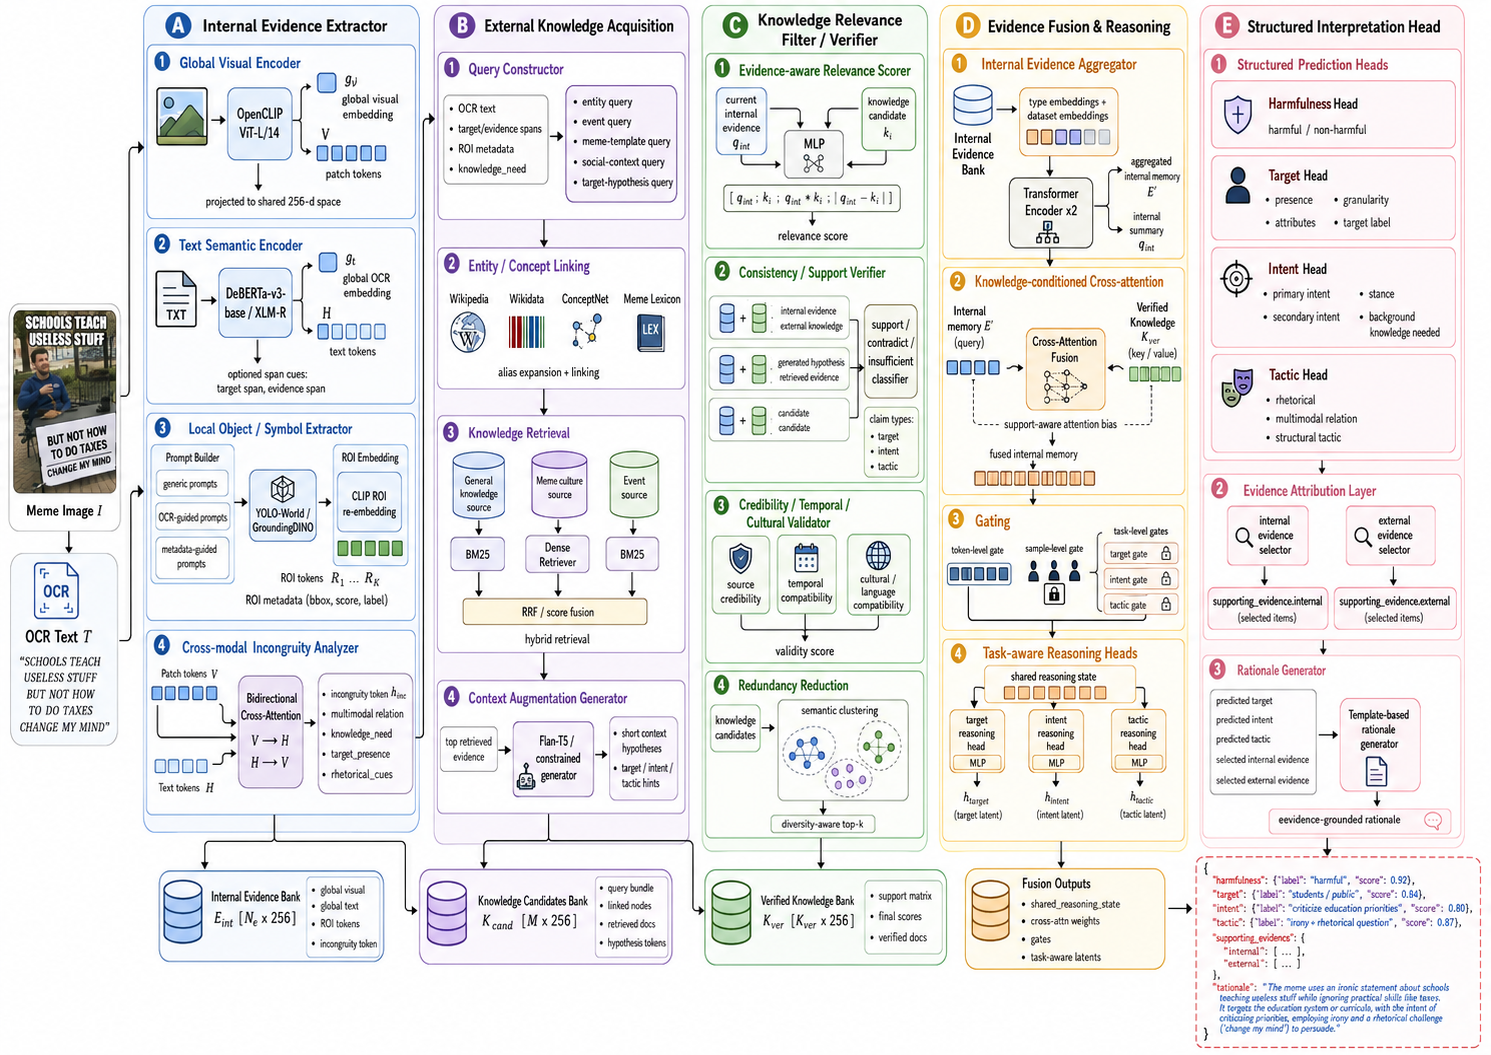
\includegraphics[width=\textwidth]{figures/manual/framework_architecture.png}
    \caption{
    Overview of our framework for evidence-grounded structured harmful meme interpretation.
    The framework consists of five stages:
    (A) internal evidence extraction,
    (B) external knowledge acquisition,
    (C) knowledge relevance filtering and verification,
    (D) evidence fusion and task-aware reasoning, and
    (E) structured interpretation with evidence attribution and rationale generation.
    This figure is a temporary project-stage visualization and will be replaced by the final camera-ready architecture figure.
    }
    \label{fig:framework_overview}
\end{figure*}

\subsection{Framework Overview}
\label{sec:method:overview}

Given a meme $\mathcal{M}=(I,T)$ consisting of an image $I$ and OCR text $T$, our framework first extracts internal evidence directly from the meme.
It then retrieves external contextual knowledge that may help interpret implicit targets, socio-cultural references, or event-dependent meanings.
Because retrieved knowledge is often noisy, outdated, or only weakly related to the meme, we explicitly filter and verify external candidates before using them.
The verified knowledge is fused with internal evidence through task-aware reasoning modules, and the final stage produces structured outputs for harmfulness, target, intent, and tactic, along with supporting evidence and an evidence-grounded rationale.

Formally, the overall pipeline can be written as

\begin{equation}
\mathcal{E}^{\mathrm{int}} = f_A(I,T),
\end{equation}

\begin{equation}
\mathcal{K}_{\mathrm{cand}} = f_B(I,T,\mathcal{E}^{\mathrm{int}}),
\end{equation}

\begin{equation}
\mathcal{K}_{\mathrm{ver}} = f_C(I,T,\mathcal{E}^{\mathrm{int}},\mathcal{K}_{\mathrm{cand}}),
\end{equation}

\begin{equation}
\mathbf{z} = f_D(\mathcal{E}^{\mathrm{int}},\mathcal{K}_{\mathrm{ver}}),
\end{equation}

\begin{equation}
\hat{\mathcal{Y}}, \hat{\mathcal{A}} = f_E(\mathbf{z}),
\end{equation}

where $\mathcal{E}^{\mathrm{int}}$ denotes internal evidence,
$\mathcal{K}_{\mathrm{cand}}$ denotes external knowledge candidates,
$\mathcal{K}_{\mathrm{ver}}$ denotes verified external knowledge,
$\mathbf{z}$ denotes fused task-aware latent representations,
$\hat{\mathcal{Y}}$ denotes structured predictions, and
$\hat{\mathcal{A}}$ denotes attribution outputs including selected evidence and rationale.

\subsection{Stage A: Internal Evidence Extractor}
\label{sec:method:stage_a}

The purpose of Stage A is to extract evidence directly observable from the meme itself.
This stage captures not only unimodal information from the image and text, but also localized symbolic cues and cross-modal incongruity patterns that are central to meme interpretation.

\paragraph{Global visual encoding.}
We first encode the meme image $I$ using a visual backbone to obtain a global visual representation and patch-level visual tokens:

\begin{equation}
\mathbf{g}_v, \mathbf{V} = \mathrm{VisualEncoder}(I),
\end{equation}

where $\mathbf{g}_v \in \mathbb{R}^{d}$ is the global image embedding and
$\mathbf{V} \in \mathbb{R}^{n_v \times d}$ is the set of patch tokens.

\paragraph{Text semantic encoding.}
The OCR text $T$ is encoded by a text encoder to produce a global text representation and token-level text embeddings:

\begin{equation}
\mathbf{g}_t, \mathbf{H} = \mathrm{TextEncoder}(T),
\end{equation}

where $\mathbf{g}_t \in \mathbb{R}^{d}$ is the global text embedding and
$\mathbf{H} \in \mathbb{R}^{n_t \times d}$ is the token sequence.

\paragraph{Local object and symbol extraction.}
Many harmful memes rely on localized visual cues such as logos, gestures, cultural symbols, or specific entities.
To capture such evidence, we apply region-level extraction and obtain a set of ROI tokens:

\begin{equation}
\mathbf{R} = \{ \mathbf{r}_1, \ldots, \mathbf{r}_K \}, \quad \mathbf{r}_k \in \mathbb{R}^{d}.
\end{equation}

Each ROI is associated with metadata such as bounding box, detector confidence, and tentative category label.

\paragraph{Cross-modal incongruity analysis.}
A key property of memes is that meaning often emerges from the tension between image and text rather than from either modality alone.
We therefore model cross-modal incongruity by allowing bidirectional interaction between visual and textual tokens:

\begin{equation}
\mathbf{C} = \mathrm{CrossModalAnalyzer}(\mathbf{V}, \mathbf{H}),
\end{equation}

where $\mathbf{C}$ denotes cross-modal evidence such as irony, contradiction, target cues, and rhetorical mismatch patterns.

Finally, Stage A outputs an internal evidence bank

\begin{equation}
\mathcal{E}^{\mathrm{int}} =
\left\{
\mathbf{g}_v, \mathbf{g}_t, \mathbf{V}, \mathbf{H}, \mathbf{R}, \mathbf{C}
\right\}.
\end{equation}

\subsection{Stage B: External Knowledge Acquisition}
\label{sec:method:stage_b}

Some memes cannot be interpreted reliably from internal content alone.
For example, the meme may reference a public event, a political actor, a culture-specific phrase, or a stereotype whose harmfulness depends on outside context.
Stage B therefore retrieves auxiliary contextual knowledge conditioned on the meme and the internal evidence extracted in Stage A.

\paragraph{Query construction.}
We build a query bundle from OCR text, detected entities, ROI metadata, target-related spans, and knowledge-need cues estimated from internal evidence.
This yields multiple query types, such as entity queries, event queries, social-context queries, and target-hypothesis queries.

\paragraph{Entity and concept linking.}
To improve retrieval specificity, extracted mentions are linked or expanded through entity and concept resources.
This step helps bridge lexical variation, aliases, and implicit references.

\paragraph{Knowledge retrieval.}
Given the query bundle, we retrieve candidate evidence from external sources.
The retriever may access general encyclopedic sources, meme-related culture resources, and event-oriented knowledge sources.
The retrieved results are aggregated into a candidate set

\begin{equation}
\mathcal{K}_{\mathrm{cand}} = \{ k_1, \ldots, k_M \}.
\end{equation}

\paragraph{Context augmentation generation.}
In addition to raw retrieved passages, we optionally generate short contextual hypotheses or compressed summaries that reformulate the retrieved evidence into meme-relevant interpretations.
These generated candidates are treated as knowledge candidates rather than trusted evidence.

\subsection{Stage C: Knowledge Relevance Filter / Verifier}
\label{sec:method:stage_c}

External retrieval is useful but noisy.
A candidate may be topically adjacent yet irrelevant to the meme, temporally outdated, culturally mismatched, or even contradictory to the meme’s actual implication.
Stage C explicitly verifies external knowledge before allowing it to influence downstream reasoning.

\paragraph{Evidence-aware relevance scoring.}
Each knowledge candidate $k_i$ is scored with respect to the current internal evidence:

\begin{equation}
s_i^{\mathrm{rel}} = \mathrm{RelScore}(\mathcal{E}^{\mathrm{int}}, k_i).
\end{equation}

This step estimates whether the candidate is genuinely relevant to the meme interpretation problem.

\paragraph{Consistency and support verification.}
Relevant candidates are then examined for whether they support, contradict, or insufficiently relate to the internal evidence and current task hypotheses.
This step is especially important because a retrieved passage may mention the same entity while still failing to support the intended target, intent, or tactic interpretation.

\paragraph{Credibility, temporal, and cultural validation.}
We further assess whether the source is credible and whether the information is temporally and culturally compatible with the meme context.
This is crucial for event-sensitive or community-specific memes.

\paragraph{Redundancy reduction.}
Finally, we cluster or rank candidates to reduce redundancy and retain a compact verified set:

\begin{equation}
\mathcal{K}_{\mathrm{ver}} \subseteq \mathcal{K}_{\mathrm{cand}}.
\end{equation}

The verified knowledge bank preserves provenance metadata such as origin, score, and support type, enabling later attribution.

\subsection{Stage D: Evidence Fusion and Task-Aware Reasoning}
\label{sec:method:stage_d}

Stage D combines internal evidence and verified external knowledge into task-sensitive latent representations.
Rather than fusing all information uniformly, we adopt a task-aware reasoning design because harmfulness, target identification, intent inference, and tactic recognition often depend on different subsets of evidence.

\paragraph{Internal evidence aggregation.}
Internal evidence is first aggregated into a contextual memory representation:

\begin{equation}
\mathbf{E}^{\mathrm{int}} = \mathrm{AggInt}(\mathcal{E}^{\mathrm{int}}).
\end{equation}

\paragraph{Knowledge-conditioned cross-attention.}
We then fuse internal memory with verified knowledge through cross-attention:

\begin{equation}
\mathbf{E}^{\mathrm{fused}} =
\mathrm{CrossAttn}(\mathbf{E}^{\mathrm{int}}, \mathcal{K}_{\mathrm{ver}}).
\end{equation}

This allows the model to selectively integrate contextual knowledge where it improves interpretation.

\paragraph{Task-aware gating.}
Not all tasks require the same amount or type of evidence.
For example, harmfulness may often rely on broad multimodal signals, whereas target interpretation may depend more strongly on entity-level or background cues.
We therefore use gating functions that modulate evidence flow at token, sample, and task levels:

\begin{equation}
\mathbf{z}^{(q)} = \mathrm{Gate}_q(\mathbf{E}^{\mathrm{fused}}), \quad q \in \mathcal{Q},
\end{equation}

where $\mathcal{Q}$ denotes the task set.

\paragraph{Task-aware reasoning heads.}
From the gated shared memory, we derive task-specific latent states for target-, intent-, and tactic-oriented reasoning.
These latent states are not yet final predictions; rather, they provide specialized representations used by the structured interpretation head.

\subsection{Stage E: Structured Interpretation Head}
\label{sec:method:stage_e}

Stage E converts the fused task-aware representations into structured predictions, evidence attribution outputs, and a concise rationale.

\paragraph{Structured prediction heads.}
We use dedicated output heads for harmfulness, target, intent, and tactic.
These heads jointly produce the structured output defined in Section~\ref{sec:problem}.
Concretely, the framework predicts:
(i) harmfulness,
(ii) target presence and target granularity,
(iii) primary intent, and
(iv) rhetorical tactic and multimodal relation.

\paragraph{Evidence attribution layer.}
To improve interpretability, we separately select supporting internal and external evidence for each prediction.
This yields attribution sets such as

\begin{equation}
\hat{\mathcal{A}}^{\mathrm{int}} \subseteq \mathcal{E}^{\mathrm{int}},
\qquad
\hat{\mathcal{A}}^{\mathrm{ext}} \subseteq \mathcal{K}_{\mathrm{ver}}.
\end{equation}

These selected items are serialized as supporting evidence rather than only being used implicitly inside the model.

\paragraph{Rationale generation.}
Finally, we generate a concise rationale conditioned on the predicted labels and selected evidence.
The rationale is designed to summarize why the meme was interpreted in a particular way, while remaining grounded in the extracted evidence and verified knowledge.

\subsection{Training Objective}
\label{sec:method:training}

The framework is trained in a multi-task manner.
Let $\mathcal{Q}$ denote the set of supervised tasks and let $m_n^q$ be a binary supervision mask indicating whether task $q$ is valid for sample $n$.
The overall objective is

\begin{equation}
\mathcal{L}
=
\sum_{q \in \mathcal{Q}}
\lambda_q \mathcal{L}_q,
\end{equation}

where $\lambda_q$ is the task weight and $\mathcal{L}_q$ is the loss for task $q$.
We use cross-entropy losses for single-label tasks and binary cross-entropy for multi-label rhetorical tactic prediction.
Masked supervision is applied so that ignored or unavailable labels do not contribute to the loss.

In addition to prediction outputs, the framework preserves structured metadata about evidence provenance, gating behavior, and attribution sources.
These records are not treated as primary prediction targets, but they are essential for later auditing, error analysis, and evidence-grounded evaluation.
\section{Experimental Setup}
\label{sec:setup}

\subsection{Datasets and Cross-Dataset Protocol}
\label{sec:setup:datasets}

We evaluate all supervised methods under a source-to-target
cross-dataset protocol.
The source collection is the HarMeme family, which combines the
COVID-19 and U.S.\ politics domains while retaining their original
domain identities.
The COVID-19 domain contains 3,544 memes and the politics domain
contains 3,469 memes, resulting in 7,013 source samples.
The normalized Facebook Hateful Memes collection, hereafter
\emph{FHM}, contains 9,000 samples and is used exclusively as a
held-out target benchmark.
Table~\ref{tab:dataset_protocol} summarizes the dataset roles.

\begin{table}[t]
    \centering
    \small
    \caption{Dataset roles in the cross-dataset protocol.
    FHM is excluded from every development decision and is used
    only for final held-out evaluation.}
    \label{tab:dataset_protocol}
    \begin{tabular}{lllr}
        \toprule
        Dataset & Family & Role & Samples \\
        \midrule
        Harm-C   & HarMeme & Train/validation & 3,544 \\
        Harm-P   & HarMeme & Train/validation & 3,469 \\
        FHM      & FHM     & Held-out test    & 9,000 \\
        \bottomrule
    \end{tabular}
\end{table}

We construct a single immutable source split using approximately
80\% of HarMeme for training and 20\% for validation.
The split is stratified jointly by the original source domain
(Harm-C or Harm-P) and the binary harmfulness label.
The split seed is fixed to 42 and is independent of the model
initialization seeds.
Every model, baseline, ablation, and knowledge condition uses the
same source split.
The resulting sample assignments and their cryptographic hashes are
stored in persistent split manifests.

FHM is not used for training, validation, early stopping,
checkpoint selection, hyperparameter search, threshold selection,
calibration, prompt development, few-shot demonstration selection,
retrieval-index construction, or knowledge-source selection.
For retrieval-based methods, the labeled meme index is constructed
from the HarMeme training partition only.
All model and decoding decisions are frozen before inference on
FHM.
Memotion is retained in the repository for future experiments but
is disabled in the current protocol because its unified
harmfulness labels require additional validation.

% TODO_CITATION: Add the authoritative HarMeme and FHM citations
% using the final BibTeX keys in reference.bib.

\subsection{Annotation and Supervision}
\label{sec:setup:annotations}

For harmfulness detection, HarMeme and FHM use their original
binary dataset labels as normalized harmful and non-harmful
supervision.
Structured target, intent, and tactic fields are obtained from the
existing schema-validated normalized annotations.
For source training, we use the \texttt{clean} normalized label
set and retain only labels that satisfy the field-specific validity
and confidence policy.

The supervised structured fields are target presence, target
granularity, primary intent, rhetorical tactic, and multimodal
relation.
Harmfulness, target presence, target granularity, primary intent,
and multimodal relation are single-label tasks.
Rhetorical tactic prediction is multi-label.
For every field, labels marked as ignored, unknown, or otherwise
invalid under the canonical vocabulary are excluded through an
explicit supervision mask rather than being treated as negative
instances.

The FHM structured annotations are agent-generated,
schema-validated silver annotations.
Accordingly, we report FHM target, intent, and tactic results as
\emph{silver structured evaluation} and do not describe these
labels as human-adjudicated gold.
For transparency, each structured metric is accompanied by the
number and proportion of FHM samples with valid supervision.
The original annotation payloads, normalized labels, audit flags,
confidence metadata, and label provenance remain available in the
saved prediction artifacts.

\subsection{Compared Methods}
\label{sec:setup:baselines}

We organize compared methods into three groups.

\paragraph{Unimodal and simple multimodal baselines.}
The text-only baseline encodes the OCR text with
DeBERTa-v3-base and trains a task classifier over the resulting
representation.
The image-only baseline uses the local pretrained OpenCLIP
ViT-B/32 image encoder.
The image--text concatenation baseline independently encodes the
image and OCR text, concatenates the two representations, and
applies a multilayer classifier.
We additionally consider a supervised OpenCLIP classifier that
jointly uses the image and text representations without the
evidence extraction, knowledge verification, or task-aware
reasoning components of our framework.

\paragraph{Supervised multimodal methods.}
Our experiment registry prioritizes representative harmful meme
detectors based on CLIP interaction, retrieval-guided contrastive
learning, target-aware modeling, and prompt-based implicit
knowledge.
These include HateCLIPper, RGCL, MOMENTA, and PromptHate.
Reasoning- and explanation-oriented methods such as IntMeme,
SAFE-MEME, and EXPLAINHM++ are included when an official
implementation, compatible checkpoint, and reproducible adapter are
available.
For external methods, we preserve the original architecture and
training objective and modify only the dataset input, output
serialization, and metric interfaces required by the common
HarMeme-to-FHM protocol.
Only completed runs that pass the common artifact and leakage audit
are included in final reproduced-result tables.
Literature-reported scores are stored separately from scores
reproduced under our protocol.

\paragraph{LMM, VLM, and agentic baselines.}
We register direct, chain-of-thought, retrieval-augmented, and
debate-style variants of general-purpose multimodal models.
Their prompts, demonstrations, output schemas, and decoding
policies are developed using HarMeme only.
No FHM example is used as an in-context demonstration or for
prompt selection.
API- or checkpoint-dependent methods are reported only when the
exact model version, inference configuration, and execution cost
are fixed and recorded.

\paragraph{Our model and ablations.}
We compare the complete framework against four train-time
ablations:
without external retrieval,
without task-specific support verification,
without task-aware gating, and
without structured auxiliary supervision.
The same ablation condition is applied during training, validation,
checkpoint selection, and FHM inference.
The structured-auxiliary ablation removes the target-presence and
multimodal-relation losses while retaining compatible output
serialization.

% TODO_CITATION: Insert citations for every external baseline that
% remains in the final experiment set.
% TODO_RESULT: Remove models that are not successfully reproduced.

\subsection{Implementation and Model Selection}
\label{sec:setup:implementation}

Our implementation uses a locally stored pretrained OpenCLIP
ViT-B/32 visual encoder and a locally stored
DeBERTa-v3-base text encoder.
All pretrained assets are verified before training, and their
paths, loading states, and SHA-256 hashes are recorded in each run
manifest.
OCR text is loaded from the existing dataset resources and is not
re-extracted during model training.

For our framework, all valid structured tasks are optimized jointly
using the masked multi-task objective described in
Section~\ref{sec:problem:objective}.
Single-label outputs use cross-entropy losses, whereas rhetorical
tactic prediction uses a multi-label binary classification loss.
The exact task weights, optimizer settings, learning rate, batch
size, number of epochs, early-stopping patience, and hidden
dimensions are fixed in the experiment configuration and reported
in the supplementary material.

The best checkpoint is selected using harmfulness Macro-F1 on the
HarMeme validation partition.
No FHM prediction is generated during checkpoint selection.
For rhetorical tactic decoding, a global sigmoid threshold is
selected on HarMeme validation predictions using non-\texttt{none}
Macro-F1.
Ties are resolved deterministically according to the predefined
decoding contract.
The selected threshold is then frozen and applied unchanged to
FHM.
No target-domain label is inspected while selecting the
checkpoint or decoding threshold.

We first conduct a one-seed pilot with model seed 42.
The final multi-seed evaluation uses model seeds
$\{42,52,123,777,2026\}$ while retaining the same source split.
Experiments are executed on NVIDIA RTX 3090 GPUs.
Each run records the resolved configuration, software environment,
pretrained asset provenance, runtime, parameter counts, peak GPU
memory, selected checkpoint, and decoding policy.

% TODO_IMPLEMENTATION: Verify the exact final optimizer,
% batch size, epoch count, and patience against the frozen
% experiment configuration before submission.

\subsection{Evaluation Metrics}
\label{sec:setup:metrics}

For harmfulness detection, the primary metric is Macro-F1.
We additionally report accuracy, precision, recall, and AUROC when
a valid binary score and both classes are available.

For target presence, target granularity, primary intent, and
multimodal relation, we report Macro-F1 over valid, non-ignored
samples.
For rhetorical tactic prediction, we report logits-only
multi-label Macro-F1 and Micro-F1.
Per-label F1, exact-match ratio, and the separate behavior of the
\texttt{none} fallback are reported in the supplementary material.
Every structured result includes its valid sample count, coverage,
unknown count, ambiguous count, and masked count.

For core ablations, we report both predictive quality and
complexity.
The latter includes total and trainable parameters, training time,
held-out inference latency, peak GPU memory, average retrieved
candidate count, and average verified knowledge count.

For multi-seed experiments, results are summarized as mean and
standard deviation.
Paired significance tests are performed only for runs sharing the
same immutable source and target manifests and the same seed set.
We do not report statistical significance from one-seed pilot
experiments.

% TODO_STATISTICS: Insert the final paired-test method and
% multiple-comparison policy after the five-seed protocol is frozen.

\subsection{Evidence, Rationale, and Verifier Assessment}
\label{sec:setup:explanation_evaluation}

We distinguish automatically measurable diagnostic properties from
human judgments of explanation quality.
Automatic diagnostics include the numbers of selected internal and
external evidence items, candidate-origin distributions, accepted
and rejected knowledge counts, evidence--rationale lexical overlap,
rationale length, provenance completeness, and rule-based
unsupported-claim indicators.
These measures are treated as analysis proxies and not as direct
proof of faithfulness.

The evaluation pipeline additionally exports human-review packages
for evidence relevance and sufficiency, rationale support and
grounding, unsupported claims, and Stage C relevance, validity, and
task-specific support.
Human-evaluation results are included only after valid annotations
have been imported and agreement checks have been completed.
Until then, the corresponding registry entries remain explicitly
marked as blocked by missing human annotation.

\subsection{Reproducibility and Artifact Audit}
\label{sec:setup:reproducibility}

Every paper-targeted run produces a resolved configuration,
environment snapshot, training log, runtime and complexity record,
validation and FHM predictions, metric file, decoding-threshold
record, and audit report.
Run manifests include hashes of the source split, target manifest,
label vocabulary, normalized annotation snapshot, configuration,
source code, and pretrained assets.

A strict audit verifies that the expected losses, prediction fields,
structured logits, decoding artifacts, model checkpoints, and
provenance records are present.
It also verifies that FHM does not occur in source training,
validation, threshold selection, few-shot demonstrations, or
retrieval indexes.
A run is considered complete for paper reporting only when all
required artifacts are present and the strict audit passes.
% !TeX root = ../main.tex
\section{Results}
\label{sec:results}

We evaluate all methods on the held-out FHM target set under the
leakage-controlled protocol in Section~\ref{sec:setup:protocol}.
Trainable models with a complete multi-seed result set are reported as
mean~$\pm$~standard deviation, whereas deterministic vision--language
baselines and canonical-seed ablations are reported as single runs.
Structured results use schema-validated FHM silver annotations and are
therefore interpreted separately from the original harmfulness labels.

We organize the empirical study around five questions:
\textbf{RQ1} whether the proposed framework improves cross-domain
harmfulness detection;
\textbf{RQ2} whether structured interpretations transfer from HarMeme to
FHM;
\textbf{RQ3} whether external knowledge is useful and whether verification
adds value beyond retrieval alone;
\textbf{RQ4} which acquired candidates are retained or rejected by the
verifier; and
\textbf{RQ5} where the framework still fails under domain shift.
RQ1--RQ2 are addressed in this section, while RQ3--RQ5 are analyzed in
Section~\ref{sec:analysis}.

\subsection{Overall Cross-Domain Performance}
\label{sec:results:harmfulness}

Table~\ref{tab:main-results} compares harmfulness detection after
development exclusively on the HarMeme source domains.
The comparison includes unimodal and simple multimodal controls,
specialized harmful-meme models, general-purpose vision--language
baselines, and our evidence-grounded framework.

\begin{table*}[t]
    \caption{
    Held-out FHM harmfulness detection under the locked
    HarMeme-to-FHM protocol.
    Multi-seed trainable methods are reported as mean~$\pm$~standard
    deviation; deterministic inference-only conditions are reported as
    single runs.
    }
    \label{tab:main-results}
    \centering
    \renewcommand{\arraystretch}{1.18}
    \begin{tabular*}{0.88\textwidth}{@{\extracolsep{\fill}}lcc@{}}
\toprule
Method & Macro-F1 & AUROC \\
\midrule
\multicolumn{3}{l}{\textit{Unimodal / simple multimodal}} \\
Text-only DeBERTa      & $0.388 \pm 0.000$ & $0.000 \pm 0.000$ \\
Image-only OpenCLIP    & $0.388 \pm 0.000$ & $0.499 \pm 0.012$ \\
Image--Text Concat     & $0.388 \pm 0.000$ & $0.000 \pm 0.000$ \\
OpenCLIP Classifier    & $0.396 \pm 0.018$ & $0.502 \pm 0.020$ \\
\addlinespace
\multicolumn{3}{l}{\textit{Specialized harmful-meme models}} \\
HateCLIPper             & $0.600 \pm 0.004$ & $0.653 \pm 0.003$ \\
MemeCLIP                 & $0.580 \pm 0.014$ & $0.643 \pm 0.009$ \\
RGCL                     & $0.564 \pm 0.021$ & $0.609 \pm 0.012$ \\
RA-HMD                   & $0.648 \pm 0.005$ & $0.691 \pm 0.009$ \\
\addlinespace
\multicolumn{3}{l}{\textit{General-purpose VLM}} \\
Qwen2.5-VL Direct        & $0.444$ & $0.745$ \\
Qwen2.5-VL Rationale     & $0.627$ & $0.734$ \\
% Pending: Qwen2.5-VL RAG is still running. This row must not survive the
% final result freeze with missing values.
Qwen2.5-VL RAG           & -- & -- \\
\addlinespace
\multicolumn{3}{l}{\textit{Proposed}} \\
% Pending: Ours requires the complete audited five-seed result set. This row
% must not survive the final result freeze with missing values.
Ours                     & -- & -- \\
\bottomrule
\end{tabular*}

\end{table*}

Among the completed trainable comparisons, RA-HMD obtains the highest mean Macro-F1
($0.648\pm0.005$) and the highest mean AUROC ($0.691\pm0.009$).
All specialized-model values are our common-protocol reproductions using
official-code adapters, not scores copied from the original papers.

The deterministic Qwen2.5-VL conditions show a different metric profile.
\textsc{Direct} obtains 0.444 Macro-F1 and 0.745 AUROC, while
\textsc{Rationale} obtains 0.627 Macro-F1 and 0.734 AUROC.
Thus, rationale prompting substantially raises hard-label Macro-F1 in this
locked comparison, whereas both conditions exceed the completed trainable
models in AUROC.  The \textsc{RAG} condition and the complete five-seed
results for our framework are still pending, so we defer overall ranking and
final interpretation until the comparison table is complete.

\subsection{Structured Interpretation}
\label{sec:results:structured}

RQ2 asks whether the model transfers more than a binary harmfulness
decision.
We therefore evaluate target presence, target granularity, primary intent,
rhetorical tactic, and multimodal relation on FHM samples with valid silver
supervision.
The five structured fields capture complementary aspects of meme
interpretation: whether a target is present, the granularity of that target,
the primary communicative intent, the rhetorical strategies expressed by the
meme, and the semantic relation between image and text.
Because these annotations are schema-validated silver labels rather than
independently adjudicated gold annotations, we report each field separately
and evaluate only samples marked valid for that field.
This prevents missing or uncertain structured supervision from being treated
as an incorrect prediction.

\begin{table*}[t]
    \caption{
    Structured interpretation on schema-validated FHM silver annotations.
    Metrics are computed only over samples with valid field-level
    supervision; valid-sample counts and coverage are reported in the
    supplementary material.
    }
    \label{tab:structured-results}
    \centering
    \begin{tabular*}{0.95\textwidth}{@{\extracolsep{\fill}}lccccc@{}}
\toprule
Method & Target-P & Target-G & Intent & Tactic & MM-Rel\\
\midrule
Not run & -- & -- & -- & -- & -- \\
\bottomrule
\end{tabular*}

\end{table*}

% TODO_RESULT:
% After result freeze, summarize:
% - which structured fields transfer most reliably;
% - which fields are hardest under domain shift;
% - whether the task-specific methods and VLM baselines show different
%   strengths across fields;
% - coverage caveats where relevant.
%
% Main table target schema:
% Method | Target-P | Target-G | Intent | Tactic | MM-Rel
% Use Macro-F1 in the main paper; move tactic Micro-F1, exact match, and
% per-label results to the supplementary material.

% !TeX root = ../main.tex
\section{Analysis}
\label{sec:analysis}

\subsection{Does External Knowledge Need Verification?}
\label{sec:analysis:verification}

RQ3 examines two related questions: whether external knowledge helps under
cross-domain transfer and whether retrieved context should be verified
before it influences the prediction.
We therefore compare the complete model with four controlled train-time
ablations under the same source split, target manifest, and canonical model
seed.

\begin{table*}[t]
    \caption{
    Controlled component ablations on held-out FHM.
    All variants use the canonical seed 42 and are interpreted as diagnostic
    comparisons rather than multi-seed significance estimates.
    }
    \label{tab:ablations}
    \centering
    \renewcommand{\arraystretch}{1.18}
    \begin{tabular*}{0.98\textwidth}{@{\extracolsep{\fill}}lcccccc@{}}
\toprule
Variant & Harm. & Target-P & Target-G & Intent & Tactic & MM-Rel \\
\midrule
% Pending rows must be resolved before the final result freeze.
Ours Full                & -- & -- & -- & -- & -- & -- \\
w/o Retrieval            & 0.473 & 0.228 & 0.099 & 0.057 & -- & 0.174 \\
w/o Support Verifier     & -- & -- & -- & -- & -- & -- \\
w/o Task-Aware Gate      & -- & -- & -- & -- & -- & -- \\
w/o Structured Auxiliary & -- & -- & -- & -- & -- & -- \\
\bottomrule
\end{tabular*}

\end{table*}

The most direct comparison is among the full model,
\textsc{w/o Retrieval}, and \textsc{w/o Support Verifier}.
The first comparison tests whether external context contributes beyond the
internal meme evidence.
The second tests whether simply acquiring external context is sufficient,
or whether task-specific verification provides additional value before
fusion.
The remaining ablations probe whether task-aware routing and structured
auxiliary supervision contribute beyond the external-knowledge pathway.

% TODO_RESULT:
% Interpret Full vs w/o Retrieval vs w/o Support Verifier first.
%
% Case A:
%   Full > w/o Support Verifier > w/o Retrieval
%   -> external context helps, and verification provides additional benefit.
%
% Case B:
%   Full > w/o Retrieval > w/o Support Verifier
%   -> unverified context is sufficiently noisy that using it can be worse
%      than relying on internal evidence alone.
%
% Do not infer multi-seed significance from these canonical-seed ablations.
%
% Final main ablation table target:
% Variant | Harm. | Target-P | Target-G | Intent | Tactic | MM-Rel
% Use Macro-F1 for the six columns; move AUROC and secondary metrics to
% supplementary material.

\subsection{What Does the Verifier Filter?}
\label{sec:analysis:verifier_flow}

RQ4 asks whether Stage~C changes the acquired candidate pool in a meaningful
way rather than acting as a nominal intermediate module.
We analyze the evidence flow from acquisition to verification using the
serialized provenance records.
For each meme, we measure the number of acquired candidates, the number
retained as verified knowledge, the number rejected, and the resulting
acceptance rate.
Where available, we additionally inspect the distribution of candidate
origins and task-specific support states.

These statistics complement the predictive ablation above.
The ablation measures whether verification changes downstream performance,
whereas the candidate-flow analysis characterizes \emph{how} the verifier
changes the information available to the reasoning stage.
Because verifier acceptance is only a model-side screening decision, we do
not interpret it as proof that an accepted candidate is factually correct.

For each meme, we summarize verifier behavior using four primary quantities:
the number of acquired candidates, the number retained as verified evidence,
the number rejected, and the acceptance rate, defined as the fraction of
acquired candidates retained after verification.
We additionally stratify these statistics by candidate origin and, when
available, by task-specific support for target, intent, and rhetorical-tactic
prediction.
All statistics are computed post hoc from the serialized provenance records;
the retrieval corpus, candidate generation procedure, and verification policy
are not modified for this analysis.

% TODO_RESULT:
% Add a compact table or figure only after the audited post-hoc export is
% available. Preferred main-paper statistics:
%
%   acquired candidates / meme
%   verified candidates / meme
%   rejected candidates / meme
%   acceptance rate
%
% Optional if space permits:
%   target-support rate
%   intent-support rate
%   tactic-support rate
%   candidate-origin distribution
%
% Detailed provenance, score distributions, and per-source diagnostics go to
% supplementary material.

\subsection{Structured Effects and Failure Modes}
\label{sec:analysis:structured_errors}
\label{sec:analysis:evidence}

RQ2 and RQ5 concern how the framework behaves beyond binary harmfulness and
where it still fails under domain shift.
We jointly examine the per-task structured results from
Table~\ref{tab:structured-results}, the
\textsc{w/o Task-Aware Gate} and
\textsc{w/o Structured Auxiliary} ablations, and the held-out error cases.
This analysis tests whether components designed for heterogeneous evidence
requirements affect particular structured fields rather than only the
aggregate harmfulness decision.

We also inspect serialized evidence and rationale diagnostics, including
selected-evidence provenance, evidence--rationale overlap, provenance
completeness, and rule-based unsupported-claim indicators.
These quantities are used only as diagnostic properties and are not treated
as direct measurements of causal faithfulness.

Held-out errors are grouped by observable failure mode, including
insufficient contextual knowledge, target confusion, cultural or
event-specific ambiguity, image--text incongruity, rhetorical-tactic
confusion, and irrelevant or insufficiently discriminative retrieved
context.
Representative qualitative examples are included only when they add
information beyond the quantitative error summary; otherwise they are moved
to the supplementary material.

For descriptive error analysis, each inspected case is assigned to the most
directly observable failure category using the model prediction, the
corresponding silver structured annotation, and the serialized evidence
record.
These categories are used to organize recurring failure patterns rather than
as an additional source of ground-truth supervision, and a case is not used
to revise the model, retrieval configuration, or decoding policy.

% TODO_RESULT:
% After result freeze:
% 1. identify structured fields most affected by w/o Task-Aware Gate;
% 2. identify whether structured auxiliary supervision helps the intended
%    fields;
% 3. report the dominant error categories;
% 4. retain only one concise rationale/evidence observation in the main paper
%    unless it materially strengthens the verifier analysis.

% !TeX root = ../main.tex

\section{Ethical Considerations}
\label{sec:ethics}

\paragraph{Exposure to harmful content.}
The datasets used in this study contain memes that may include
hateful, discriminatory, misogynistic, offensive, politically
sensitive, or otherwise disturbing content.
Researchers who inspect raw memes, retrieved evidence, generated
rationales, or error cases may therefore be exposed to potentially
harmful material.
We minimize unnecessary exposure by separating automated
experiments from manual review, limiting qualitative inspection to
samples required for validation or analysis, and avoiding the
inclusion of gratuitous harmful examples in the paper.
Any future human evaluation should provide annotators with an
explicit content warning, allow them to pause or withdraw, and
avoid requiring repeated exposure to particularly severe content.

\paragraph{Dataset provenance and privacy.}
We use existing meme benchmarks according to their intended
research purposes and retain their original sample identifiers,
dataset families, and domain metadata.
The source protocol combines the COVID-19 and U.S.\ politics
domains of HarMeme for training and validation, while FHM is used
only as a held-out target dataset.
We do not use FHM samples for training, prompt development,
threshold selection, retrieval-index construction, or any other
model-selection decision.

Memes may contain identifiable people, public figures, usernames,
logos, or contextual references.
Our task is content-level harmfulness interpretation rather than
person identification.
The framework does not attempt to infer private identity,
demographic attributes, or sensitive personal information beyond
what is explicitly required by the dataset annotation schema.
Any public release of code or experiment manifests should avoid
redistributing raw images unless permitted by the licenses and
terms of the original datasets.

% TODO_ETHICS: Verify the final redistribution and licensing policy
% of every dataset before releasing code or artifacts.

\paragraph{Annotation provenance and uncertainty.}
The harmfulness labels used in this study originate from the
respective source benchmarks.
The target, intent, and tactic annotations are produced through the
existing structured annotation pipeline and are preserved with
their confidence, audit flags, masks, and provenance metadata.
In particular, the current structured annotations for FHM are
agent-generated, schema-validated silver annotations rather than
human-adjudicated gold labels.
We therefore report the corresponding results as
\emph{silver structured evaluation} and provide field-level
coverage and valid-sample counts.

Automated annotation may reproduce the cultural assumptions,
social biases, and systematic errors of the underlying models.
Labels such as harmfulness, intent, and rhetorical tactic may also
admit multiple reasonable interpretations.
We retain explicit \texttt{ambiguous}, \texttt{unknown}, and
masked states where defined by the annotation protocol, rather than
forcing every sample into a confident category.
Human-evaluation results are not reported unless independently
collected annotations have been validated and imported through the
designated evaluation procedure.

\paragraph{External knowledge and contextual bias.}
External contextual information can help interpret implicit
references, but it may also be incomplete, outdated, culturally
specific, or factually incorrect.
Retrieved passages, generated hypotheses, and fallback candidates
are therefore stored as distinct candidate types and are not
treated as verified knowledge by default.
The Stage C verifier filters candidates according to relevance,
validity, and task-specific support; however, this procedure does
not constitute a guarantee of factual correctness.

Knowledge sources may disproportionately represent dominant
languages, regions, institutions, or political perspectives.
Consequently, a system that relies on external retrieval may
perform unevenly across communities or cultural contexts.
We retain source and candidate provenance to make such failures
auditable and include cultural-context errors in the planned error
analysis.

\paragraph{Rationale limitations.}
Generated rationales are intended to make model decisions easier
to inspect, not to provide authoritative factual explanations.
A rationale may be fluent while still omitting relevant context,
overstating weak evidence, or introducing an unsupported claim.
For this reason, rationale text is not used as the formal source of
target, intent, or tactic predictions.
Formal structured metrics are computed from trainable model
outputs, while rationale quality is evaluated separately through
grounding, support, and unsupported-claim analyses.

The evidence attribution and attention traces retained by the
framework should also not be interpreted as causal explanations.
They are diagnostic records that indicate which evidence was
selected or emphasized by the implemented pipeline.

\paragraph{Risks of automated moderation.}
False positives may incorrectly flag satire, criticism, political
speech, or benign humor, whereas false negatives may allow harmful
content to remain undetected.
Errors may be especially consequential for marginalized groups,
whose language and cultural references are often underrepresented
in training data.
Accordingly, the proposed framework should not be deployed as an
autonomous moderation authority.
Its predictions, evidence records, and rationales are better viewed
as decision-support information for trained human moderators.

The structured outputs should likewise not be used to assign intent
or harmful attributes to individuals outside the context of the
analyzed meme.
Model confidence does not remove the need for human review,
particularly in ambiguous, culturally dependent, or high-impact
cases.

\paragraph{Dual-use considerations.}
The same analysis capabilities that support moderation research
could be misused to identify weaknesses in content-moderation
systems or to create memes designed to evade detection.
To reduce this risk, released artifacts should prioritize model
interfaces, evaluation protocols, and aggregated results rather than
unnecessary reproduction of harmful material.
We also avoid presenting retrieved or generated harmful content as
endorsed factual information.

\paragraph{Human evaluation and oversight.}
The current automated pipeline can export annotation packages for
evidence relevance, rationale quality, verifier decisions, and
stage-level error analysis.
It does not generate human gold judgments automatically.
Any future human evaluation should use informed participation,
clear annotation guidelines, appropriate compensation, secure data
handling, and a process for resolving annotator disagreements.
Institutional review or ethics approval requirements should be
determined before such evaluation is conducted.

% TODO_ETHICS: Add the final human-evaluation protocol, annotator
% demographics at an aggregate level, compensation policy, and
% institutional review status if human evaluation is performed.
\section{Conclusion}
\label{sec:conclusion}

We cast harmful meme understanding as a structured,
evidence-grounded interpretation problem instead of only a binary
classification task.
The proposed framework jointly models harmfulness, target presence and
granularity, primary communicative intent, rhetorical tactics, and
multimodal relation while retaining an auditable record of the evidence
available to the prediction.

The framework decomposes this process into five stages:
internal multimodal evidence extraction, external knowledge acquisition,
knowledge verification, task-aware evidence fusion, and structured
interpretation with evidence attribution.
In particular, separating knowledge acquisition from verification prevents
retrieved or generated contextual information from being treated
automatically as trusted evidence, while provenance records preserve the
distinction among acquired, verified, rejected, and selected information.

We evaluate this formulation under a leakage-controlled cross-dataset
protocol in which models are developed only on HarMeme and evaluated on the
held-out Facebook Hateful Memes benchmark after model, retrieval, prompt,
and decoding decisions have been frozen.
Beyond the original harmfulness labels, schema-validated silver
annotations enable separate analysis of target, intent, rhetorical tactics,
and multimodal relation while making annotation coverage and provenance
explicit.

% TODO_RESULT:
% Replace this paragraph after the final audited result freeze.
% It should contain only 2--3 observations actually supported by the final
% tables, for example:
%
% Across the held-out target set, [Ours/result statement].
% The component analysis further shows that [retrieval/verifier/gate result].
% Structured evaluation indicates that [most/least transferable field].
%
% Do not introduce SOTA, statistical significance, or efficiency claims
% unless directly supported by the final audited experiments.

Taken together, this work provides a modular basis for studying not only
whether a meme is harmful, but also which structured interpretation the
model produces and what evidence was permitted to influence that decision.
The current results should nevertheless be interpreted in light of the
silver structured annotations, dataset-specific cultural coverage, and the
diagnostic rather than causal nature of the retained evidence and
rationales.
Future work can extend the protocol with independently adjudicated
structured annotations, broader cultural and linguistic domains, and
human-centered evaluation of evidence usefulness and rationale quality.


\bibliographystyle{ACM-Reference-Format}
\bibliography{reference}

\end{document}
